\documentclass[a4paper,11pt]{article}

\usepackage[T1]{fontenc}
\usepackage[utf8]{inputenc}
\usepackage[english,swedish]{babel}


%% Sets page size and margins
\usepackage[a4paper,top=3cm,bottom=2cm,left=3cm,right=3cm,marginparwidth=1.75cm]{geometry}

%% Useful packages
\usepackage{amsmath}
\usepackage{graphicx}
\usepackage{blindtext}
\usepackage[colorinlistoftodos]{todonotes}
\usepackage[colorlinks=true, allcolors=blue]{hyperref}
\usepackage{float}
\usepackage{caption}
\usepackage{subcaption}
\captionsetup[subfigure]{width=0.95\linewidth}

\title{FMAF25: Projekt 2}
\author{Adham Sakhnini \\ Emil Johansson \\ Jonna Johansson \\ Kristoffer Lundgren}

\begin{document}

\maketitle

%\begin{abstract}
%Your abstract.
%\end{abstract}

\section{Inledning}

Studiens syfte har varit att analysera ett nyframtaget malariaprofylax genom att dels försöka beskriva dess kinetik och dels bestämma en lämplig dosering av profylaxet, givet kliniska data. Den kinetiska beskrivningen innefattar bland annat att profylaxets farmakokinetiska parametrar bestäms, variationen mellan individer beskrivs och ett terapeutiskt intervall för profylaxets koncentration i blodet bestäms. I doseringsdelen behandlas även individuella strategier, utifall den rekomenderade dosen inte fungerar för en individ.

Malaria är en mycket allvarlig sjukdom som orsakas av parasiter som kommer in i blodomloppet via myggstick~\cite{ann}. Den är mycket utbredd i Afrika men finns även i Sydamerika och Asien. Vanliga symptom är bland annat  hög feber, frossa, muskelvärk och illamående. Det finns även vissa sorters malaria som orsakar medvetslöshet, chock och svår diarré. Dessutom kan sjukdomen vara mycket länge ty parasiter kan fnnas kvar i kroppen i flera år. Om den ej behandlas kan den vara dödlig; varje år dör flera hundratusen människor i malaria, där majoriteten är barn~\cite{lennart}.

Ett vanligt sätt  att förebygga malaria är med malariaprofylax, tabletter som skyddar i det fall man blir stucken. Sådan medicin rekomenderas därför vanligen till resenärer som ska till områden där malaria finns. Det finns flera olika sorters malariamedel som fungerar något olika, de varierar bland annat i hur länge och hur ofta man bör ta dem. De flesta bör tas under hela vistelsen samt efter hemkomst, en del behövs dock tas även innan avresa. De olika profylaxen varierar också i styrka på biverkningar, huruvida man kan ta dem om man ammar eller är gravid samt vilka andra läkemedel som går att ta samtidigt som profylaxet~\cite{malariaab}.

%därför har detta och detta testats för att hitta en bra dos som skyddar mot malaria men inte ger för mycket biverkningar och det kommer att diskuteras i denna rapport 


\section{Metod}
Den erhållna kliniska datan utgörs av mätningar via blodprov av plasmakoncentrationer av profylaxet vid olika tidpunkter för 10 patienter efter intag av en bolusdos i form av tre tabletter om 5 mg styck. Vid tidpunkterna för blodproven har patienterna även självrapporterat upplevda biverkningar. Vid tidigare \emph{in vitro}-försök har man kommit fram till att koncentrationen bör hållas över 1mg/L för att skyddet mot malarian ska vara tillräkligt starkt~\cite{horisto}. För att kunna bearbeta denna data och beskriva kinetiska parametrar behövs sedan någon form av fördelningsmodell för profylaxet, där en tvåbehållarmodell har valts (de två behållarna kan tänkas utgöras av blodomloppet respektive organvävnad), av skälen att det är en något mer träffsäker modell än en enbehållarmodell samtidigt som den är tillräckligt enkel att behandla matematiskt. Det har visat sig att den observerade datan går att passa väldigt bra till en tvåbehållarmodell. Detta ger ett system av differentialekvationer enligt
\begin{align}
C'(t) & = a(t) + k_{pc}C_p(t) - (k_{cp}+k_{ce})C(t) \\
C_p '(t) & = k_{cp}C(t) - k_{pc}C_p(t)
%satans alignmiljö
\label{eq1}
\end{align}
där $a(t)$ anger absorptionshastigheten, $C(t)$ plasmakoncentrationen, $C_p(t)$ organkoncentrationen och respektive $k$ utgör hastighetskonstanter. Absorptionshastigheten antas sedan vara enkel, det vill säga att en tablett i magen sönderfaller med en hastighet som är proportionell mot hur mycket av den som finns kvar, vilket ger 
\begin{equation}
a(t) = F k_a e^{-k_a t}
\label{eq2}
\end{equation}
där $F$ anger hur mycket av tabletten som tas upp. Ekvation (\ref{eq2}) ger sedan tillsammans med $C(0) = C_0$ och $C_p(0) = 0$ (bolus dos) att plasmakoncentrationen får utseendet 
\begin{equation}
C(t) = \frac{Fk_a A}{k_a - \lambda}(e^{-\lambda t} - e^{-k_a t}) + \frac{Fk_a B}{k_a - \mu}(e^{-\mu t} - e^{-k_a t}).
\label{eq3}
\end{equation}
för tvåbehållarmodellen. För att göra passning av data till ekvation (\ref{eq3}) möjlig behöver dock konstanterna $F$ och $A$ respektive $F$ och $B$ buntas ihop, där med fördel även $k_a$, $\lambda$ samt $\mu$ förs in, till nya konstanter. Modellen blir då
\begin{equation}
C(t) = A'(e^{-\lambda t} - e^{-k_a t}) + B'(e^{-\mu t} - e^{-k_a t})
\label{eq4}
\end{equation}
med $A' = Fk_a A/(k_a - \lambda)$ samt $B' = Fk_a B/(k_a - \mu)$.

Med en modell på plats i form av ekvation (\ref{eq4}) passades så datan (där koncentrationerna först delades med tre för att få fram effekten från en tablett, vilket är vad som framöver refereras till som ``en dos'') för de olika patienterna ur ett minsta kvadrat-perspektiv via Nelder-Meads algoritm (vilken finns implementerad i funktionen \texttt{fminsearch} i \texttt{Matlab}) för att bestämma de olika konstanterna för respektive patient, avrundade till fyra decimaler.
\begin{table}[H]
\centering
\caption{Tabell över de skattade konstanterna i ekvation (\ref{eq4}) där varje rad motsvarar respektive patient.}
\label{tab1}
\begin{tabular}{lllll}
$A'$   & $B'$   & $k_a$  & $\lambda$ & $\mu$  \\ \hline
0.1782 & 3.0547 & 0.5000 & 0.0200    & 0.2456 \\
0.2092 & 2.0028 & 0.5000 & 0.0200    & 0.1348 \\
0.1734 & 2.1412 & 0.5000 & 0.0200    & 0.2137 \\
0.1256 & 2.5083 & 0.5000 & 0.0200    & 0.2501 \\
0.1177 & 1.0821 & 0.4996 & 0.0201    & 0.1820 \\
0.1943 & 1.7237 & 0.5001 & 0.0200    & 0.1843 \\
0.1633 & 2.1943 & 0.5000 & 0.0200    & 0.2432 \\
0.1829 & 2.5645 & 0.5000 & 0.0200    & 0.2274 \\
0.7180 & 5.3203 & 0.5000 & 0.0200    & 0.1643 \\
0.4153 & 4.2136 & 0.5000 & 0.0200    & 0.1847
\end{tabular}
\end{table}
Från tabell (\ref{tab1}) inses ganska lätt att variansen hos $k_a$ och $\lambda$ är tämligen låg, varför dessa bektraktas som konstanta mellan individer. För $\mu$ finns förvisso en liten varians, men $\mu$ valdes ändå att bektrakta som konstant. $A'$ och $B'$ uppvisar däremot ett nämvärt stokastiskt beteende och undersökningar genom olika tester (Jargue-Bera, Lilliefors samt Kolmogorov-Smirnov) får oss att dra slutsatsen att dessa är (nästan) normalfördelade. Detta möjliggör konstruktionen av ett prediktionsintervall för patientresponsen hos en okänd individ. Med $A' \sim N(\mu_{A'}, \sigma_{A'}^2)$ respektive $B' \sim N(\mu_{B'}, \sigma_{B'}^2)$ så erhålles väntevärde och varians för plasmakoncentrationen i ekvation (\ref{eq4}) enligt nedan. Det gäller att summor av normalfördelade stokastiska variabler också är normalfördelade. Vi får
\begin{align}
\mathrm{E}[C(t)] & = \mathrm{E}[A'(e^{-\lambda t} - e^{-k_a t})\} + \mathrm{E}\{B'(e^{-\mu t} - e^{-k_a t})] \nonumber \\
& = \mu_{A'}(e^{-\lambda t} - e^{-k_a t}) + \mu_{B'}(e^{-\mu t} - e^{-k_a t}),
\label{eq5}
\end{align}
samt
\begin{align}
\mathrm{Var}[C(t)] & = \mathrm{Var}[A'(e^{-\lambda t} - e^{-k_a t}) + B'(e^{-\mu t} - e^{-k_a t})] \nonumber \\ 
& =  \mathrm{Var}[A'(e^{-\lambda t} - e^{-k_a t})] + \mathrm{Var}[B'(e^{-\mu t} - e^{-k_a t})] \nonumber \\
& + 2(e^{-\lambda t} - e^{-k_a t})(e^{-\mu t} - e^{-k_a t})\mathrm{Cov}[A',B'] \nonumber \\ 
& = (e^{-\lambda t} - e^{-k_a t})^2\mathrm{Var}[A'] + (e^{-\mu t} - e^{-k_a t})^2\mathrm{Var}[B'] \nonumber \\
& +  2(e^{-\lambda t} - e^{-k_a t})(e^{-\mu t} - e^{-k_a t})\mathrm{Cov}[A',B'] \nonumber \\ 
& = (e^{-\lambda t} - e^{-k_a t})^2\sigma_{A'}^2 + (e^{-\mu t} - e^{-k_a t})^2\sigma_{B'}^2 \nonumber \\
& +  2(e^{-\lambda t} - e^{-k_a t})(e^{-\mu t} - e^{-k_a t})\mathrm{Cov}[A',B'].
\label{eq6}
\end{align}
Ett prediktionsintervall med konfidensgrad $p$ fås då av
\begin{equation}
I_p = \mu \pm t_n s \sqrt{1 + 1/n}
\label{eq7}
\end{equation}
där $t_n$ är den $p$:te percentilen i $t$-fördelningen med $n-1$ frihetsgrader och $\mu$ och $s$ är det skattade väntevärdet respektive standardavvikelsen för $C(t)$. Under förutsättning att dosresponsen har linjärt beteende (vilket är ett rimligt antagande under förutsättning att transport- och metaboliseringsprocesser inte är mättade) så kan simulering av doseringar betraktas helt additivt\footnote{Eller med ett finare ord: ``superposition''.}. Detta tillsammans med vetskap om hur prediktionsintervallet för plasmakoncentrationerna genom ekvation (\ref{eq7}) möjliggör doseringssimuleringar för att fastställa en rekommendation för hur profylaxet ska tas.

\section{Resultat}
De till en dos normaliserade plasmakoncentrationerna efter en bolusdos av malariaprofylaxet återfinns grafiskt i figur (\ref{fig1}) tillsammans med en passning enligt ekvation (\ref{eq4}) för respektive patient. Värdena för respektive patients konstanter återfinns i tabell (\ref{tab1}).
\begin{figure}[H]
\centering
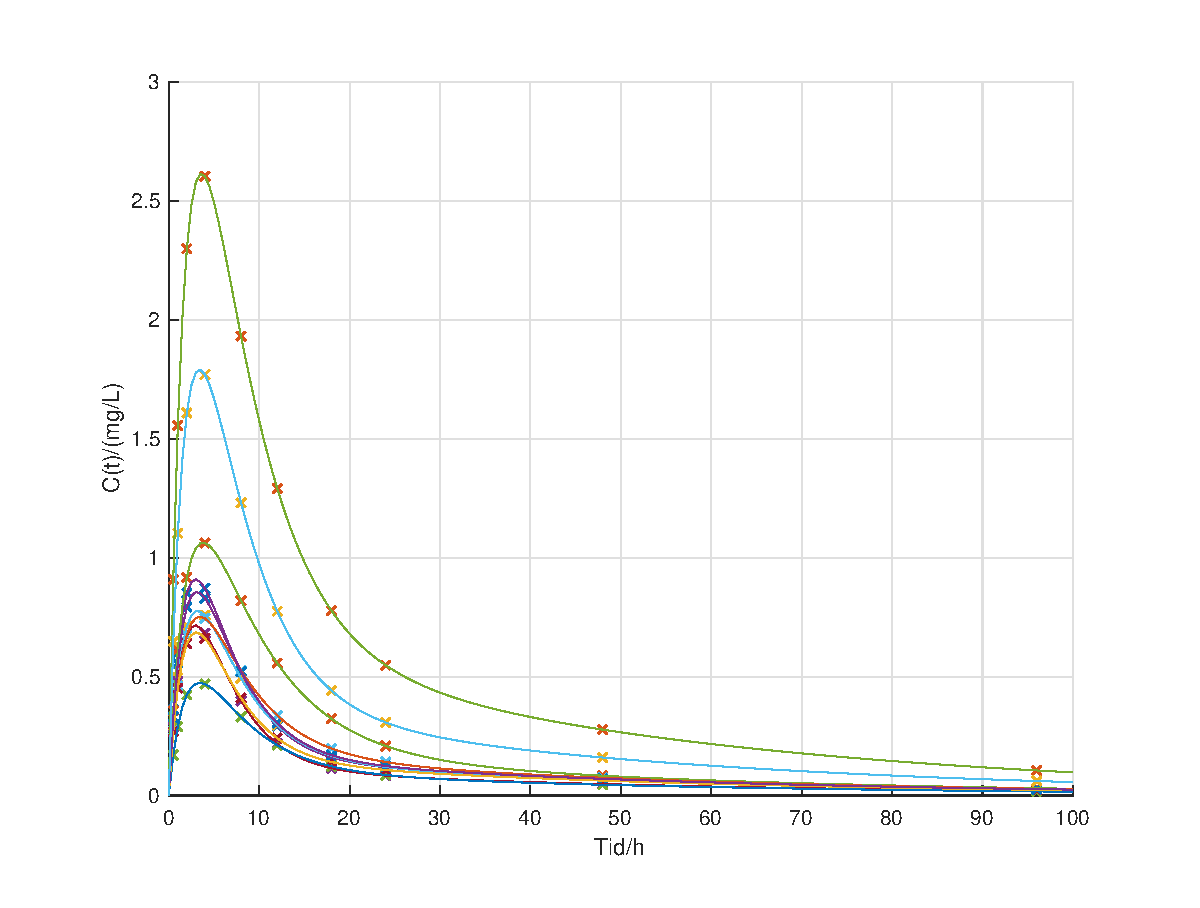
\includegraphics[width=0.6\textwidth]{fig1.eps}
\caption{\label{fig1}Uppmätta plasmakoncentrationer av malariaprofylaxet efter bolusdos (markerade som ``x'') samt passningar av ekvation (\ref{eq4}) (markerade med helstreckad linje) till dessa koncentrationer.}
\end{figure}
De upplevda biverkningarna, vilka graderas mellan 0 till 4 enligt tabell (\ref{tab2}), återfinns plottade i figur (\ref{fig2}).
\begin{table}[H]
\centering
\caption{Tabell över biverkningar}
\label{tab2}
\begin{tabular}{l|llll}
Nivå         & 0    & 1     & 2        & 3     \\ \hline
Biverkningar & inga & milda & moderata & svåra
\end{tabular}
\end{table}
\begin{figure}[H]
\centering
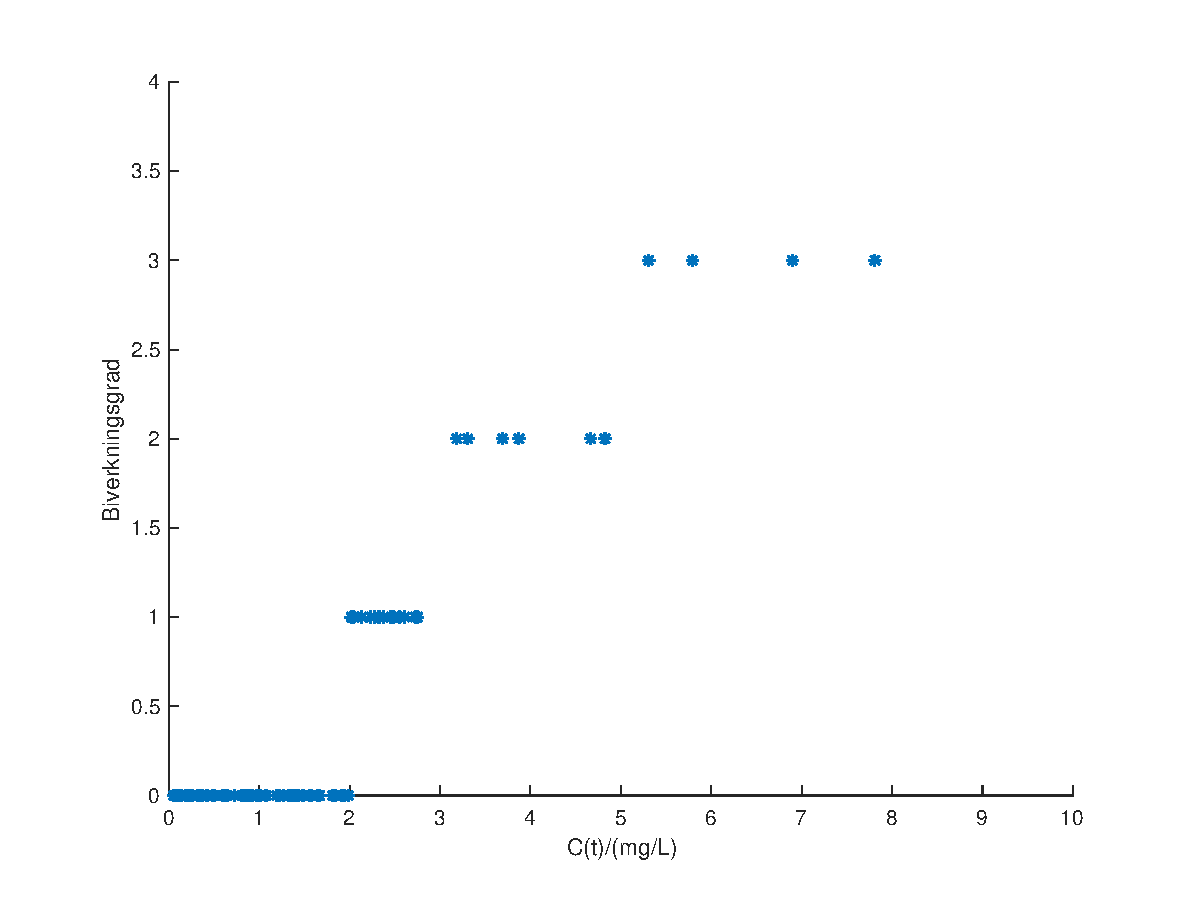
\includegraphics[width=0.6\textwidth]{fig2.eps}
\caption{\label{fig2}Biverkningsnivå som funktion av plasmakoncentration av malariaprofylaxet.}
\end{figure}
Från figur (\ref{fig2}) syns tydliga brytgränser för biverkningsnivåerna, varför dessa inte analyseras djupare än via en okulärbesiktning; biverkningsgrad 0 inträffar i intervallet 0-2 mg/L i blodplasman av profylaxet, biverkningsgrad 1 i intervallet 2-3 mg/L, biverkningsgrad 2 i intervallet 3-5 mg/L samt biverkningsgrad 3 i intervallet 5 mg/L och uppåt. Företaget bakom profylaxets intention var att doseringen skulle utgöras av en tablett var 12:e timme. En simulering av plasmakoncentrationerna för detta schema återfinns i figur (\ref{fig3}), där prediktionsintervallet beräknas enligt ekvation (\ref{eq7}).
\begin{figure}[H]
\centering
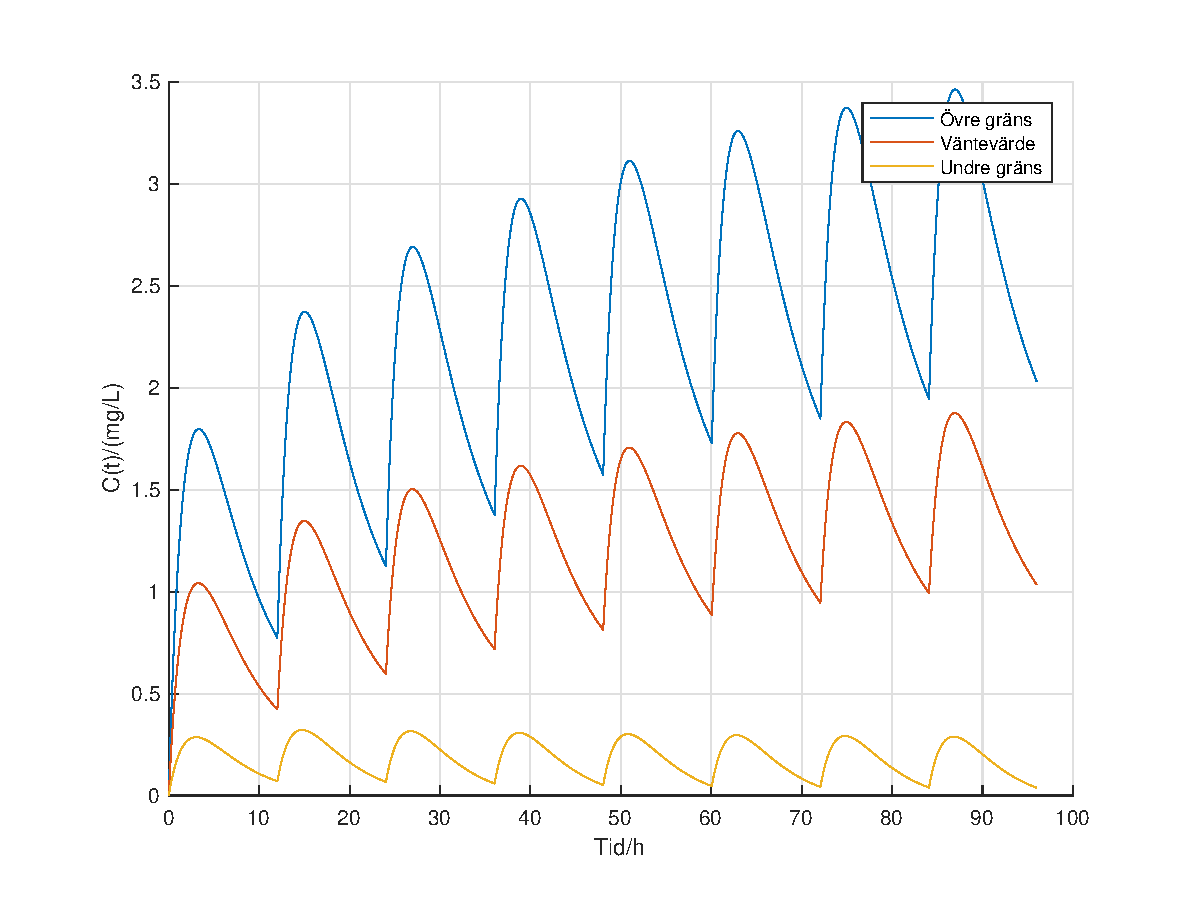
\includegraphics[width=0.6\textwidth]{fig3.eps}
\caption{\label{fig3}Simulering av plasmakoncentrationen av malariaprofylaxet med ett 80\%-igt prediktionsintervall, där en tablett tas var 12:e timme.}
\end{figure}
Som synes i figur (\ref{fig3}) kommer koncentrationen av profylaxet med ganska låg sannolikhet att befinna sig över 1 mg/L större delen av tiden vid denna dosering, vilket man från \textit{in vitro}-studier vet är den undre gränsen för profylaxkoncentrationen för att det ska vara verksamt. Det tar dessutom lång tid innan någon form av steady state inträder, vilket innebär att konsumtion av profylaxet behöver inledas lång tid innan individen kan förväntas utsätta sig för malariasmitta. Baserat på ett antal olika simuleringar, där kriterierna att schemat ska vara realiserbart under en normal sömncykel, profylaxkoncentrationen ska företrädesvis hålla sig över 1 mg/L större delen av tiden samt att profylaxet inte ska behöva intas långt tidigare än avresa så är vår rekommendation att inta tre tabletter 12 timmar innan avresa och därefter ta två tabletter var 12:e timme. Figur (\ref{fig4}) illustrerar den förväntade profylaxkoncentrationen med ett 80\%-igt prediktionsintervall.
\begin{figure}[H]
\centering
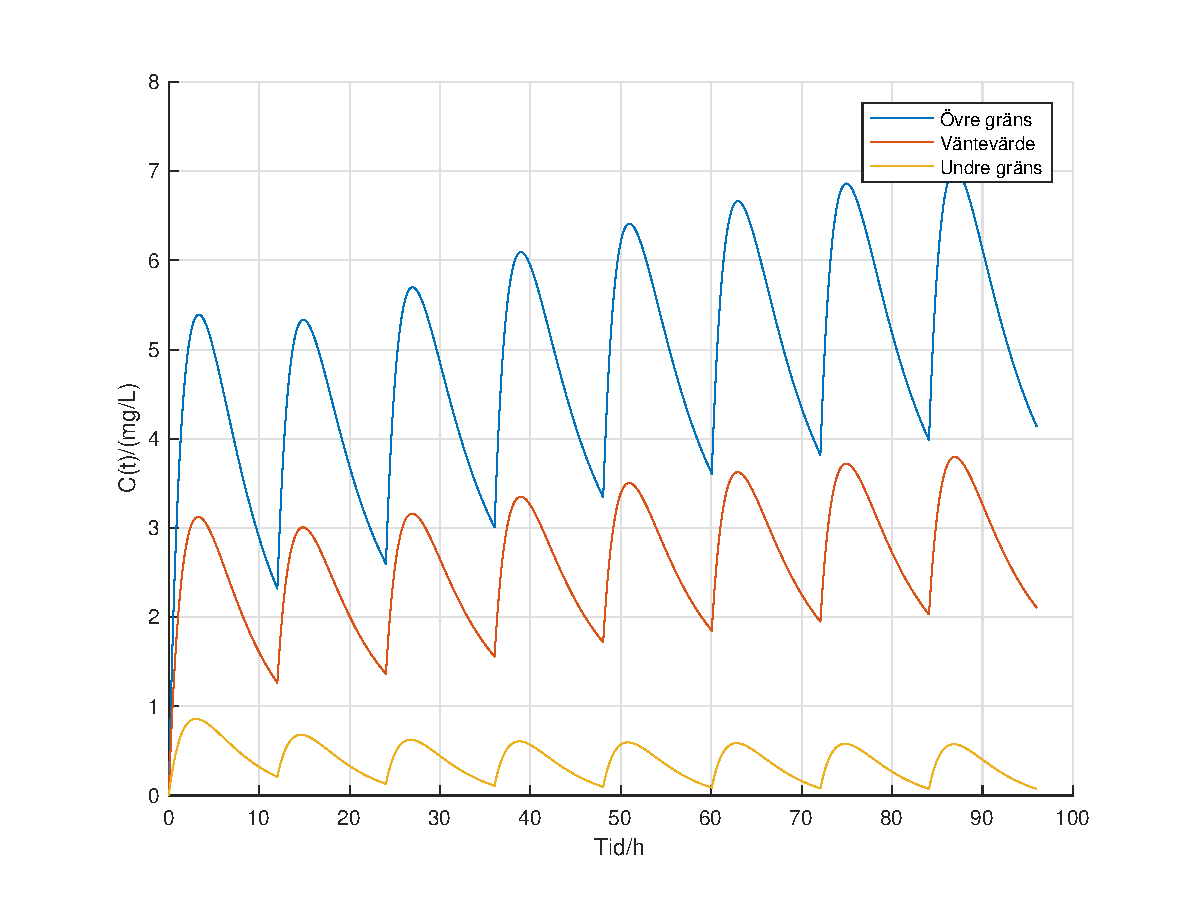
\includegraphics[width=0.6\textwidth]{fig4.eps}
\caption{\label{fig4}Simulering av plasmakoncentrationen av malariaprofylaxet med ett 80\%-igt prediktionsintervall, där tre tabletter tas 12 timmar innan avfärd, därefter två tabletter var 12:e timme. Koncentrationen ligger större delen av tiden över 1 mg/L.}
\end{figure}
Hänsyn behöver även tas till biverkningar. Med doseringsschemat illustrerat i figur (\ref{fig4}) bör de flesta få en profylaxkoncentration under 3 mg/L, men en viss stigande trend kan observeras. Skulle biverkningsnivå 2 upplevas rekommenderar vi därför att sänka dosen till en tablett var 12:e timme. Vid biverkningsnivå 3 rekommenderar vi att sänka dosen en tablett var 24:e timme och när biverkningsnivå 2 är nådd fortsätta med en tablett var 12:e timme. Figur (\ref{fig5}) illustrerar dessa utfall.
\begin{figure}[H]
\centering
\begin{subfigure}[t]{.5\textwidth}
    \centering
    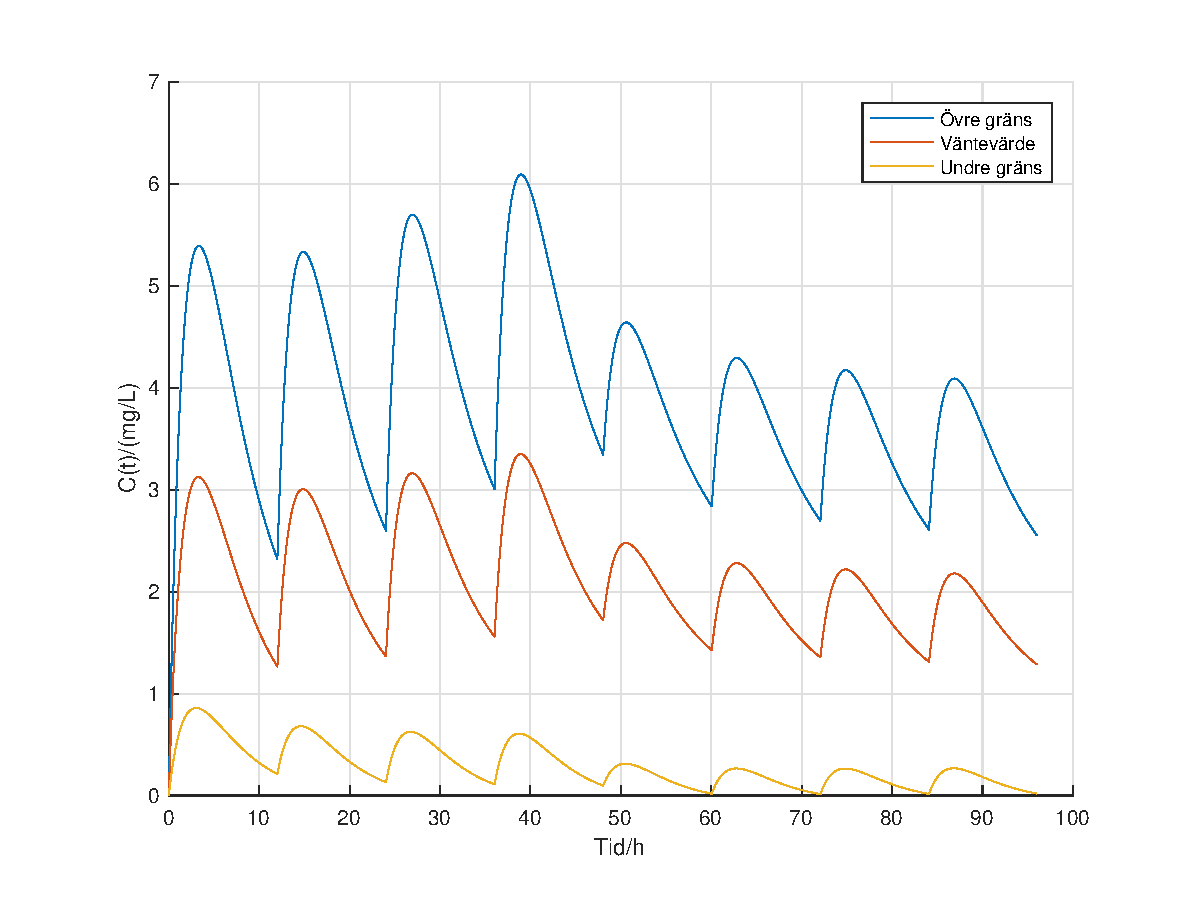
\includegraphics[scale=0.3]{fig5a.eps}
    \caption{Biverkningsnivå 2 nådd och vid 48 timmar efter medicineringsstart sänks dosen till en tablett var 12:e timme.}
    \label{fig5a}
\end{subfigure}% 
\begin{subfigure}[t]{.5\textwidth}
    \centering
    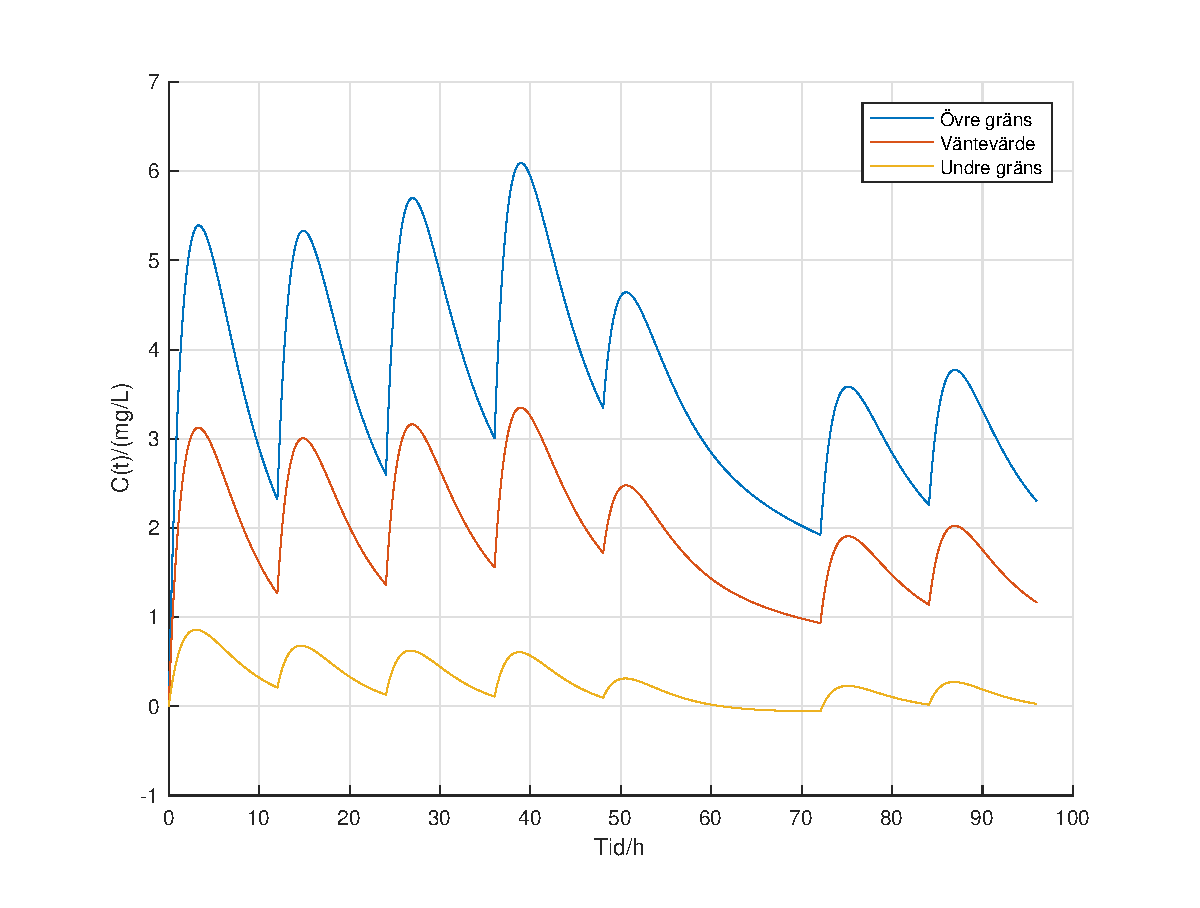
\includegraphics[scale=0.3]{fig5b.eps}
    \caption{Biverkningsnivå 3 nådd och vid 48 timmar efter medicineringsstart sänks dosen till en tablett var 24:e timme, för att vid biverkningsnivå 2 övergå till en tablett var 12:e timme.}
    \label{fig5b}
\end{subfigure}
\caption{Illustration av förändringar i doseringsschema som konsekvens av biverkningar.}
\label{fig5}
\end{figure}

\section{Diskussion}
% Andra lösningar?
Det finns förutom den dosering som valts många andra doseringar som är rimliga dygnsmässigt och uppfyller de givna  kraven. Anledningen till att det är dosen i figur \ref{fig4} som rekomenderas är att denna dos snabbt kommer upp i en acceptabel koncentration i blodet vilket dels innebär att profylaxet inte behöver tas långt innan avresa, vilket kan innebära en längre period av biverkningar, dels att det kan användas vid eventuella oförutsägbara händelser genom att snabbt minimera skador. 

% Anledningar till variation? Individuella + tillfälliga (+felkällor?)
Som nämnts under resultat varierar koncentrationen av den aktiva substansen i blodet kraftigt mellan individer. Detta beror med stor sannolikhet på biologiska skillnader hos individerna så som hur stort upptaget av den aktiva substansen är, vikt, ålder och kön. Det kan dock vara värt att notera att det är möjligt att variationen beror på tillfälliga skillnader, till exempel om en individ nyligen ätit, drucket eller sovit. Detta innebär att individer som har högt upptag och upplever biverkningar en gång inte nödvändigtvis kommer att fortsätta göra det vid framtida doser. 




% Vad göra om svåra biverkningar
%Om svåra biverkningar dock skulle uppstå bör en halvering av dosen rekomenderas då det förmodligen gäller en individ med hög upptagningsförmåga. Således innebär en halvering att denna individ kommer att hamna innom det godkända intervallet för koncentration profylax i blodet.

Värt att nämna om prediktionsintervallet är att det är gjort med enbart tio mätpunkter, vilket ger totalt $9$ frihetsgrader i skattningen. Eftersom att variansen i plasmakoncentrationen även är hög så ger det ett väldigt brett intervall där man för höga konfidensnivåer får sannolikhet för negativa plasmavärden (se figur \ref{fig5a}). Detta är naturligtvis inte realistiskt och beror på att modellen inte definierar någon undre gräns på vilka nivåer som är tillåtna. Dessuom har vi i studien antagit, motiverat av några statistiska tester, en normalfördelning hos parametrarna $A'$ och $B'$ i uttrycket (\ref{eq5}) för plasmakoncentration. Detta har gjorts framför allt för att på ett enkelt sätt kunna konstruera ett analytiskt uttryck för ett intervall där de flesta patienter bör hamna, men inducerar problemet med att det inte finns någon undre plasmagräns. Vi noterar vidare att parametrarna enbart visade sig vara svagt normalfördelade och för att få en mer robust skattning vore det önskvärt att erhålla en större datamängd.    

% Förslag till vidare studier? + Prat om slump? Tänk: rapport en avsedd för t.ex. läkare
Givet den insamlade datan så kan den ovan beskrivna doseringen anses nå tillfredsställande resultat. Trots detta bör fler studier göras på profylaxet innan det når marknaden: med endast tio deltagare i studien kan resultatet påverkats såväl av ett icke representativt urval av individer, som rena tillfälligheter. Dessutom har ingen data tagits fram för hur länge efter hemkomst profylaxet behöver tas för att utgöra ett säkert skydd. Fortsatta studier av profylaxet är därför att rekommendera. I dessa studier föreslås även orsaker till individuell variation undersökas ytterligare. Till exempel kan samband mellan faktorer som vikt, ålder och kön och upptagningsförmåga av profylaxet undersökas. Detta skulle kunna leda till att mer individuell dosering skulle bli möjlig, vilket minskar både risken att få svåra biverkningar och risken att få malaria. 


\begin{thebibliography}{9}
\bibitem{ann}
  Ann Tisiimeks, \emph{Småkryp, ohyra och annat äckelpäckel}, Guttamåla: förlaget Förlaget, 1632.
\bibitem{lennart}
  Lennart Schmepel, "Lite ditt och datt om malaria och sånt", \emph{Saker som kan döda en}, vol 666, nr 37, s. 8-402, Juni 2019.
\bibitem{malariaab}  
  Malaria AB, \emph{So you think you have malaria?}, Veberöd: Antons förlag, 1991. 
\bibitem{horisto}
  Horisto Malarone, "Jag gjorde en undersökning på ett malariaprofylax och här är resultaten", \emph{Allt om keramik (och malaria)}, vol 1, nr 1, s. 1, Januari 2001.
\end{thebibliography}


% \subsection{How to include Figures}

% First you have to upload the image file from your computer using the upload link the project menu. Then use the includegraphics command to include it in your document. Use the figure environment and the caption command to add a number and a caption to your figure. See the code for Figure \ref{fig:frog} in this section for an example.

% \begin{figure}
% \centering
% \includegraphics[width=0.3\textwidth]{frog.jpg}
% \caption{\label{fig:frog}This frog was uploaded via the project menu.}
% \end{figure}

% \subsection{How to add Comments}

% Comments can be added to your project by clicking on the comment icon in the toolbar above. % * <john.hammersley@gmail.com> 2016-07-03T09:54:16.211Z:
% %
% % Here's an example comment!
% %
% To reply to a comment, simply click the reply button in the lower right corner of the comment, and you can close them when you're done.

% Comments can also be added to the margins of the compiled PDF using the todo command\todo{Here's a comment in the margin!}, as shown in the example on the right. You can also add inline comments:

% \todo[inline, color=green!40]{This is an inline comment.}

% \subsection{How to add Tables}

% Use the table and tabular commands for basic tables --- see Table~\ref{tab:widgets}, for example. 

% \begin{table}
% \centering
% \begin{tabular}{l|r}
% Item & Quantity \\\hline
% Widgets & 42 \\
% Gadgets & 13
% \end{tabular}
% \caption{\label{tab:widgets}An example table.}
% \end{table}

% \subsection{How to write Mathematics}

% \LaTeX{} is great at typesetting mathematics. Let $X_1, X_2, \ldots, X_n$ be a sequence of independent and identically distributed random variables with $\text{E}[X_i] = \mu$ and $\text{Var}[X_i] = \sigma^2 < \infty$, and let
% \[S_n = \frac{X_1 + X_2 + \cdots + X_n}{n}
%       = \frac{1}{n}\sum_{i}^{n} X_i\]
% denote their mean. Then as $n$ approaches infinity, the random variables $\sqrt{n}(S_n - \mu)$ converge in distribution to a normal $\mathcal{N}(0, \sigma^2)$.


% \subsection{How to create Sections and Subsections}

% Use section and subsections to organize your document. Simply use the section and subsection buttons in the toolbar to create them, and we'll handle all the formatting and numbering automatically.

% \subsection{How to add Lists}

% You can make lists with automatic numbering \dots

% \begin{enumerate}
% \item Like this,
% \item and like this.
% \end{enumerate}
% \dots or bullet points \dots
% \begin{itemize}
% \item Like this,
% \item and like this.
% \end{itemize}

% \subsection{How to add Citations and a References List}

% You can upload a \verb|.bib| file containing your BibTeX entries, created with JabRef; or import your \href{https://www.overleaf.com/blog/184}{Mendeley}, CiteULike or Zotero library as a \verb|.bib| file. You can then cite entries from it, like this: \cite{greenwade93}. Just remember to specify a bibliography style, as well as the filename of the \verb|.bib|.

% You can find a \href{https://www.overleaf.com/help/97-how-to-include-a-bibliography-using-bibtex}{video tutorial here} to learn more about BibTeX.

% We hope you find Overleaf useful, and please let us know if you have any feedback using the help menu above --- or use the contact form at \url{https://www.overleaf.com/contact}!

% \bibliographystyle{alpha}
% \bibliography{sample}

\end{document}

% 4/4 2017 - träffades första gången, bestämde vilka samverkansverktyg vi skulle använda och försökte komma överens om hur vi ska arbeta framöver 
% 21/4 2017 - träffades efter påskledigheten. Jobbade fr.a. m. parameterskattningar, fastnade lite på F, A och B. Började även prata om dosering. 
% 24/4 2017 - Efter skrivföreläsning: fortsatte på dosering, tog fram ett prediktionsintervall (efter en del möda) och en matlabmodell för flera, fördröjda doser (superposition). Styrde upp lite om vilka som skulle skriva vad. 
%26/4 2017- Gjorde färdigt det sista på modellen och redigerade inledning samt skrev  del av diskussion, metod och resultat
28/4 2017- Redigerade rapporten la till delar av diskussionen. skickade in rapporten.